\section{Stato dell'Arte}
\label{sec:stato-arte}
In questa sezione verrà descritto lo stato dell'arte dei modelli \textit{agent-based} di evacuazione da tsunami, senza focalizzarsi sui modelli di inondazione.
Successivamente alcuni lavori verranno approfonditi nelle sottosezioni seguenti, in particolare modelli \textit{network-based} con scenari multimodali.

I primi modelli di evacuazione da tsunami sono stati basati sui modelli \textit{network-based} utilizzati per l'evacuazione da altri disastri come
uragani, incendi e inondazioni \parencite{usuzawa1997development, imamura2001development}.

Uno dei primi aspetti che è stato preso in considerazione è il comportamento umano,
in particolare le reazioni dei residenti all'arrivo dello tsunami
e il tempo che ci mettono per iniziare a evacuare.

Queste informazioni sono state raccolte tramite dei questionari rivolti ai residenti
e usate per stimare i tempi di partenza dell'evacuazione \parencite{imamura2001development, saito2004simulation}.

Questi primi modelli \textit{network-based} hanno usato come regola di \textit{path finding}
proseguire verso il nodo con altitudine maggiore.
Successivamente si è passati a usare il percorso
più breve \parencite{katada2004disaster} e altre strategie di routing basate sull'apprendimento 
come Nash equilibrium e system optimal \parencite{lammel2009towards}.

Un altro aspetto importante per l'evacuazione è la conoscenza dell'ambiente da parte degli agenti.
Alcuni lavori hanno distinto gli agenti in base alla loro conoscenza e
studiato gli effetti di diverse proporzioni tra categorie di agenti.
\textcite{nguyen2012simulation} hanno definito \textit{fox agent} un pedone ben informato che segue i segnali
stradali fino a un rifugio e \textit{sheep agent} un pedone che non sa
come comportarsi e quindi segue i \textit{fox agent} o si muove casualmente.
\textcite{takabatake2017simulated} invece hanno distinto gli agenti in residenti e visitatori.
I residenti sono agenti che conoscono il percorso più breve per evacuare, mentre i visitatori
seguono gli altri scegliendo la strada con più individui o si muovono verso una zona più elevata.

Con l'aumento della potenza di calcolo è stato possibile passare da modelli \textit{network-based} a modelli \textit{grid-based} e ibridi.
Inoltre è stato possibile usare una quantità di dati maggiore e sfruttare il calcolo parallelo \parencite{wijerathne2013hpc, makinoshima2018enhancing}.

\textcite{wijerathne2013hpc} hanno proposto un modello \textit{grid-based} che utilizza un sistema di navigazione basato
sulla visione. Gli agenti si muovono verso un luogo sicuro ben visibile scegliendo la strada con una maggiore distanza di visione.
%
Anche in questo lavoro vengono distinti visitatori, che si affidano alla visione, e non-visitatori, che hanno conoscenza di un'area
limita al di fuori della quale vengono considerati visitatori.

\pagebreak

In molti modelli vengono considerati esclusivamente solo pedoni, ma alcuni lavori hanno analizzato l'aggiunta della presenza di auto e altri veicoli,
e si concentrano nella gestione delle interazioni tra i diversi tipi di agenti \parencite{goto2012tsunami, wang2016agent, wang2021novel}.

Questi modelli di evacuazione multimodale verranno approfonditi in quanto questo lavoro si focalizza sulle interazioni tra i diversi tipi di agenti.

\subsection{Goto et al. (2012)}
In questo lavoro sono stati modellati diversi tipi di agenti raggruppati in famglie: pedoni lenti, pedoni normali, motociclisti e occupanti di un'auto.
Ogni agente rappresenta una famiglia che è formata da un numero diverso di individui in base al tipo di agente.
%
La velocità dei pedoni e dei motocicli viene aggiornata in base alla densità
e sono state gestite le interazioni tra i diversi agenti all'interno di una corsia stradale e i passaggi da una corsia all'altra.

La popolazione considerata è composta da oltre 20,000 individui ed è stato assunto che tutti si trovino a casa all'inizio dell'evacuazione.
%
Gli agenti evacuano seguendo il percorso più breve verso il rifugio più vicino. 
Il percorso più breve per auto considera il tempo di attraversamento della strada, mentre per 
moto e pedoni la lunghezza della strada.

Alcuni dei rifugi prevedono una capacità limita, che nel caso venga raggiunta la capacità massima gli agenti dovranno cambiare destinazione.

Un agente colpito dallo tsunami muore quando la profondità dello tsunami supera 1 m.

\begin{figure}[ht]
    \centering
    \begin{subfigure}{0.32\textwidth}
        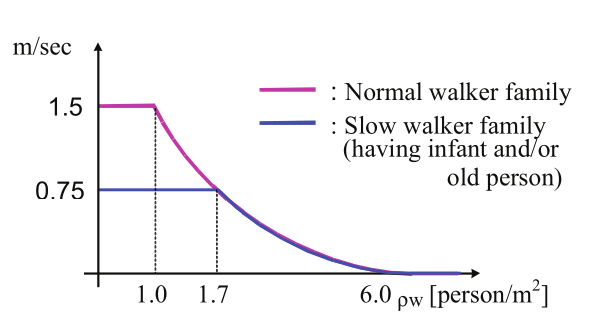
\includegraphics[width=\textwidth]{images/speed_GOTO.png}
        \caption{}
        \label{fig:goto-ped}
    \end{subfigure}
    \hfill
    \begin{subfigure}{0.32\textwidth}
        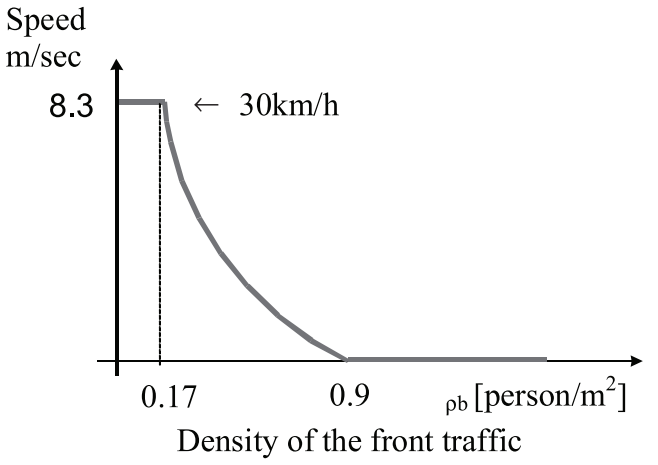
\includegraphics[width=\textwidth]{images/speed_GOTO_motocicli.png}
        \caption{}
        \label{fig:goto-moto}
    \end{subfigure}
    \hfill
    \begin{subfigure}{0.32\textwidth}
        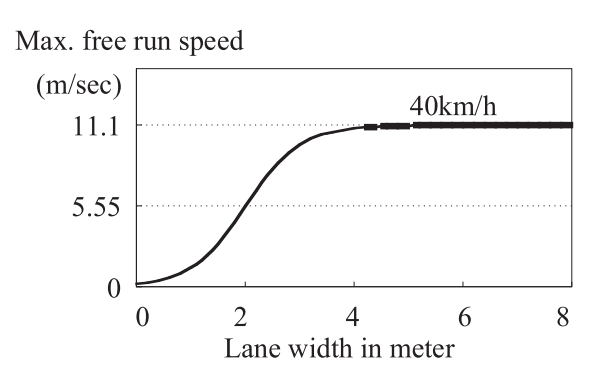
\includegraphics[width=\textwidth]{images/speed_GOTO_auto.png}
        \caption{}
        \label{fig:goto-auto}
    \end{subfigure}
    \caption{Relazione velocità-densità per i pedoni (a), per i motocicli (b), e velocità massima per le auto al variare della larghezza della strada (c).}
    \label{fig:ankdasndk}
\end{figure}

I pedoni sono distinti in \textit{normal walkers}, con velocità massima di 1.5 m/s, e
\textit{slow walkers} (famiglie con disabili, anziani o bambini), con velocità massima di 0.75 m/s.
%
La velocità viene aggiornata al variare della densità con un massimo di $6 p/m^2$ (Fig. \ref{fig:goto-ped}).

Per i motocicli è stata considerata una velocità massima di 30km/h e una densità massima di 0.9 $p/m^2$ (Fig. \ref{fig:goto-moto}).

Per pedoni e motocicli la densità viene calcolata tramite la seguente formula:
$\rho = n /(L \times W)$, dove $n$ è il numero di agenti nell'area di fronte all'agente $L \times W$, $L$ è la lunghezza di ricerca 
e $W$ la larghezza della strada.

\begin{figure}[ht]
    \centering
    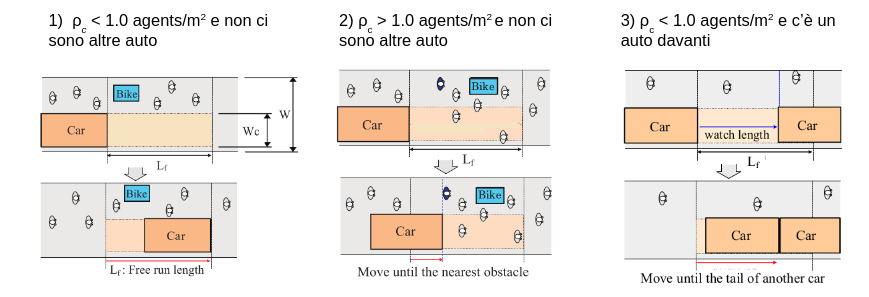
\includegraphics[width=\textwidth]{images/goto_car.png}
    \caption{Diversi casi che descrivono fino a dove l'auto si può muovere, in base alla densità e alla presenza di altre auto di fronte.}
    \label{fig:goto-car-model}
\end{figure}

Le auto in assenza di ostacoli si muovono per $L_{f} = V_{f} \times \Delta_{t} $, dove $L_{f}$ è la \textit{free run length},
$V_{f}$ la velocità massima e $\Delta_{t}$ il \textit{time step}.
La velocità massima cambia in base alla larghezza della strada con un limite di 40 km/h (Fig. \ref{fig:goto-auto}).

Per le auto la densità è definita da $\rho = n /((W - W_{c}) x L_{f})$, dove $W_{c}$ è la larghezza di un' auto.
La densità di un'auto viene considerata 10 volte quella di un pedone, mentre di una moto 2 volte quella di un pedone.

In base alla densità l'auto si muoverà fino al prossimo ostacolo, oppure fino alla prossima auto se presente (Fig. \ref{fig:goto-car-model}).

\subsection{Mostafizi, Wang et. al}
In questa sezione verrà descritto brevemente il modello di \textcite{wang2016agent} in quanto è stato scelto come modello di partenza per questo lavoro.
Inoltre verranno mostrate alcune modifiche effettuate in altri lavori degli stessi autori.

\subsubsection*{Wang et. al (2016)}

Nel lavoro di \textcite{wang2016agent} viene studiato come il tempo di preparazione, la scelta della modalità di evacuazione, la velocità dei pedoni e la 
presenza di rifugi per l'evacuazione verticale influenzi la quantità di vittime.

Al contrario del modello di \textcite{goto2012tsunami} viene considerato un numero molto limitato di agenti, ovvero 4502 individui. 
Inoltre i rifugi si assume che abbiano capacità illimitata e che non subiscano danni sismici. 

Come nel lavoro di \textcite{goto2012tsunami} il routing avviene tramite il percorso più breve e viene considerato lo stesso casualty model.

\pagebreak

Il modello gestisce due tipi di agenti: auto e pedoni. Le interazioni tra questi tipi di agenti sono limitate.
I pedoni hanno velocità costante definita secondo una distribuzione normale, e le auto interagiscono tra loro 
tramite il modello \textit{General Motors}. Quindi non è gestita nessuna interazione pedone-pedone e pedone-auto.


% Questo modello verrà descritto brevemente in quanto selezionato come modello di partenza per questo lavoro e nella sezione successiva.
% Questo modello consiste di un numero molto limitato di agenti rispetto al modello di \textcite{goto2012tsunami}, 4502 individui.
% Viene analizzato come l'aggiunta di rifugi verticali modalità
% Anche qui il routing avviene mediate l'utilizzo del percorso più breve ed lo stesso casualty model viene considerato, 
% mentre gli shelter si assume abbiano capacità illimitata.

% Al contrario di \textcite{goto2012tsunami} le interazioni tra i diversi tipi di agenti sono abbastanza limitate.
% I pedoni hanno velocità costante definita secondo una distribuzione normale, mentre le auto interagiscono tra di loro secondo il modello \textit{General Motors}.
% Infine non avendo dati sul quali fare validazione gli autori si sono limitati ad uno studio 
% dell'impatto sulla mortalità dato dai diversi parametri del modello tempi di preparazione, velocità dei pedoni e modalità di evacuazione.

\subsubsection*{Mostafizi, et. al. (2017)}
Il lavoro di \textcite{mostafizi2017agent} è basato sul precedente \parencite{wang2016agent} e si focalizza sul misurare la resilienza della rete stradale tramite l'analisi della mortalità.

Per i tempi di preparazione viene considarata una situazione ideale in cui gli agenti evacuano immediatamente dopo l'allarme. Inoltre per poter rappresentare
meglio il rischio per persone anziane o bambini, la profondità critica per il casualty model è stata ridotta a 0.5 m.

Ogni scenario è stato simulato molteplici volte per catturare la randomicità dei parametri. 
Per misurare il contributo di ogni link alla mortalità totale è stata considerata la mortalità media per ogni scenario al variare del numero di auto e pedoni.
I link critici sono stati identificati come quelli con una percentuale di mortalità superiore al 5\% sulla media di ogni combinazione di agenti.

\subsubsection*{Mostafizi, et. al. (2019)}
Il lavoro di \textcite{mostafizi2019agent} si basa sui due lavori precedenti e 
presenta un'analisi di sensitività di diversi fattori. 
In aggiunta ai precedenti lavori sono stati analizzati diversi parametri per 
il modello \textit{General Motors} e diversi limiti di velocità per le auto.


\subsection{Z. Wang e Jia (2021)}
In questo lavoro viene proposto un modello di evacuazione multimodale e una valutazione dei rischi modellando l'incertezza
nei danni sismici nelle strade e nei parametri del modello. Inoltre viene introdotta una velocità variabile per i pedoni e sono state 
gestite le interazioni tra auto e pedoni.

Sono state considerate diverse popolazioni al variare del numero di agenti: 5000 e 10,000,
che rappresentano la popolazione all'inizio dell'estate e 15,000 rappresenta il picco nella stagione estiva.

Gli agenti sono distinti in pedoni e auto ed evacuano verso il rifugio più vicino seguendo il percorso più breve.
Ogni auto contiene 4 persone ed è equivalente a 10 volte un pedone in spazio occupato.
Gli agenti per poter evacuare in auto dovranno prima raggiungere a piedi degli appositi parcheggi.

La velocità per i pedoni è distribuita secondo una normale $\mathcal{N}(\mu_p,\sigma_p)$ troncata tra 0.75 m/s e 3.83 m/s e
con $\mu_p \sim \mathcal{U}(1.4, 2)$ e $\sigma_p \sim \mathcal{U}(0.1, 0.6)$.
Inoltre viene aggiornata in base alla densità di fronte all'agente con una \textit{search length} di 4m secondo l'andamento mostrato in figura \ref{fig:wang2021}.

\begin{figure}[ht]
    \centering
    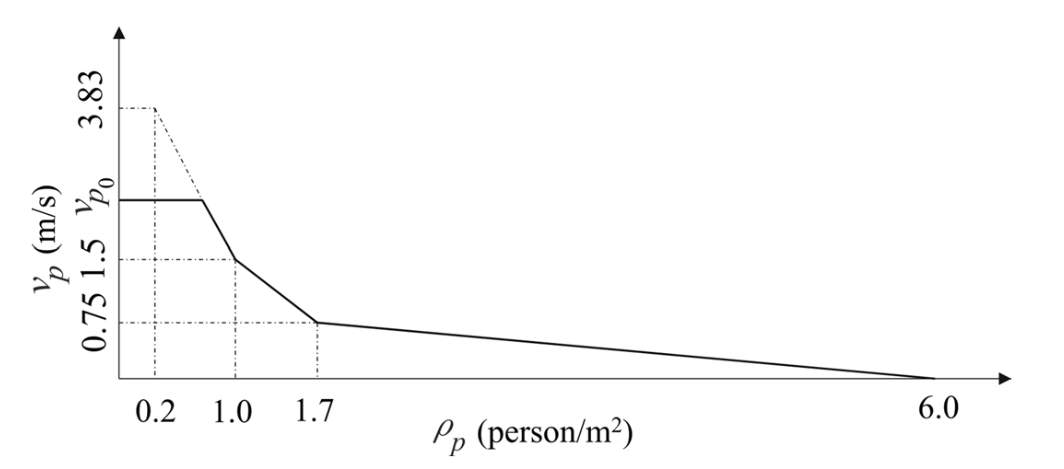
\includegraphics[width=0.7\textwidth]{images/speed_WANG.png}
    \caption{Relazione velocità-densità \textcite{wang2021novel} basato su un approssimazione del modello di \textcite{goto2012tsunami}}
    \label{fig:wang2021}
\end{figure}

Per le auto è stato utilizzato il modello di \textcite{greenshields1935study} che aggiorna la velocità in base alla densità di fronte lungo la \textit{free run length},
con una massima velocità di 40 km/h e una densità massima di 160 veh/km per i link senza restrizioni sul traffico date dai danni sismici.

Per la gestione delle interazioni tra auto e pedoni vengono definite tre fasi di traffico in base al rapporto
tra il volume dei pedoni e delle auto: \textit{vehicle-dominated}, \textit{balanced} e \textit{pedestrian-dominated}.
Al variare della fase cambia la larghezza della strada occupabile sia per pedoni che per le auto.

Per gestire i danni sismici viene assegnato un livello di distruzione ad ogni link e sulla base di questo viene 
ridotta la capacità massima riducendo la densità massima.

Per i tempi di partenza viene utilizzata la distribuzione di Rayleigh dove i parametri
invece di essere fissati seguono delle apposite distribuzioni uniformi.

Rispetto ad altri lavori che utilizzano un livello di profondità fissa per determinare la morte degli agenti, in questo lavoro
viene considerato che la profondità sia distribuita uniformemente in [0.5, 3]. 
